\documentclass[11pt]{article}
\usepackage[letterpaper]{geometry}
\usepackage{graphicx} % Required for inserting images
\usepackage{hyperref}
\usepackage{xcolor}

\hypersetup{
    colorlinks,
    allcolors={blue!20!black},
}

% hogg typesetting
\addtolength{\topmargin}{-.30in}
\addtolength{\textheight}{1.40in}
\renewcommand{\paragraph}[1]{\smallskip\par\noindent\textbf{#1}~---}
\pagestyle{myheadings}
\markright{Villar, Hogg, \& Zanna? / Improving emulators\hfill}
\setlength{\parindent}{1.3em}
\sloppy\sloppypar\raggedbottom\frenchspacing

\begin{document}\thispagestyle{empty}
\section*{\raggedright
Using geometry and physics to improve machine learning emulators}

\medskip\noindent\textbf{Soledad Villar}\\
{\footnotesize
Department of Applied Mathematics and Statistics, Johns Hopkins University}

\medskip\noindent\textbf{David W. Hogg}\\
{\footnotesize
Center for Cosmology and Particle Physics, Department of Physics, New York University}

\medskip\noindent\textbf{Laure Zanna}\\
{\footnotesize
Courant Institute, New York University}

\medskip\noindent
\textit{A white paper submitted in 2023 August to ONR Applied and Computational Analysis}

\bigskip

\paragraph{Abstract}
In most of the physical science and engineering disciplines, the principal theories are computational:
They generate predictions or explanations for data via expensive simulations.
The computational load required for many important simulation-based projects exceeds the total scientific computing capacity (!) of the United States.
Thus many projects are placing big bets on \emph{emulation}, in which an expensive simulation is replaced or augmented by a machine-learning model that is trained to replicate some aspects of the input--output relationship of the simulation, but at far lower computational cost.
Emulators have substantial limitations; the largest might be that it is hard to verify that the emulator is replicating the input--output relationship accurately; by construction full simulation-based verification isn't possible.
In this white paper, we describe two strategies that have the potential to improve trust in emulation.
In one strategy, we will build machine-learning model components---network layers---that provably obey a set of classical-physics symmetries, many of which are related to geometry.
These components make use of group-theoretic invariants in the same way that the theories of physics are written in terms of invariants.
In the other strategy, we will develop adversarial attack methodologies against emulators, based on symmetries and conservation laws, to ``red-team'' emulators used in critical tasks in scientific and engineering projects.
These adversarial methods can be used to validate models, identify weaknesses, test data augmentations and other strategies, and potentially create new training strategies.
Along the way we will apply these tools to contemporary problems in cosmology and ocean science, which are areas that depend critically on emulators for their near-term goals.

\section{What is an emulator?}
In the physical sciences and in engineering disciplines, theoretical predictions are no longer computed with pencil and paper.
In almost all mature domains, the theory is computed by complex computer simulations.
These have the property that they can deal with complex boundary conditions, and integrate nonlinear coupled equations.
Simulation cost is driven by the dimensionality of the problem, the nonlinearity of the equations involved, and the range of scales (ratio of the largest scale to the smallest scale) resolved.
In most domains, it is impossible to simulate the full observable range of scales, at the accuracy desired for precision measurement and prediction.
Simulations are necessarily run in a trade space between accuracy and computational cost; anything that speeds simulations without sacrificing resolution delivers more science from current projects.

For a specific example, two of the largest cosmology projects in the world right now are the ESA \textsl{Euclid} project to measure large-scale structure \cite{euclid} and the \textsl{Simons Observatory} project to measure the cosmic microwave background.
These projects are both simulation-limited, in the sense that the precise measurements that they will make depend on precise comparison of the data with accurate simulations representing the physical cosmological model.
It is currently impossible for either of these projects, with traditional computational methods, to do the necessary suite of simulations at sufficient accuracy and number to make measurements as precise as the data natively might permit.
Thus both projects intend to augment their simulation suites with ma\-chine-learn\-ing-gen\-er\-a\-ted emulations.

There are five different kinds of emulators in use in the physics domains with which we interact:

\paragraph{Full replacement}
The most extreme---and most standard---kind of emulator is one that simply replaces the full input--output relationship of the entire simulation.
Thus if the simulation starts with initial conditions and boundary conditions, and ends with a final state (after an integration), the full-replacement emulator would be trained to learn the full relationship between the initial and boundary conditions and the final state.
A full-replacement emulator is a complete, plug-in replacement for the simulator.

\paragraph{Integrator}
Simulation run times generally scale linearly with the number of time steps required to execute the integration.
A set of emulators can be trained on a set of snapshots of the simulation internal state at a set of times that is much smaller than the full set of integration time steps.
Each emulator is trained to learn the relationship between the internal state of the simulation at one time $t_A$ and the internal state of the simulation at a later time $t_B$, such that the emulator can be used to replace the integrator during the time interval from $t_A$ to $t_B$.
A set of such emulators can be used to replace part or all of the integration performed by the simulator.

\paragraph{Resolution translator}
Simulation run times generally scale with the number of grid points or basis functions in the representations of the state.
Thus the simulator gets faster as resolution is reduced.
An emulator can be trained to learn the relationship between a low-resolution simulation and a matched high-resolution simulation.
Then a high-resolution simulation can be emulated by running a fast low-resolution simulation and applying the learned translation.

\paragraph{Physics in-painter}
In most physical systems, there are coupled physics domains with different levels of computational complexity.
For example, in cosmology, the pure gravitational part of the simulation is relatively low in computational cost, but the baryonic part---the atoms, photons, ram pressures, magnetic fields---is very high in computational cost.
The simulator gets faster as physics domains, or equations, or interaction terms, are dropped.
An emulator can be trained to learn the relationship between a simulation with some physics dropped and a matched full simulation.
Then a full-physics simulation can be emulated by running a partial-physics simulation and applying the learned in-painting of the missing physics.

\paragraph{Statistics generator}
In many contexts, the goal of the simulation is not to produce the full state of the physical system, but only certain critical statistics, such as the two-point correlation function (in the case of some cosmology problems) or the HOGG (in the case of some ocean-science problems).
In this case, there is no need to emulate the entire simulation state.
Instead, it makes sense to train the emulator to learn only the relationship between the initial and boundary conditions of the simulation and the final statistics of particular interest.

\smallskip
One can ask, in general: \emph{Why would any emulator ever work?}
Isn't integrating the differential equations underlying the simulation with a good integrator going to be better than any machine-learning method trained on such integrations?
There are at least three answers to this question.
The first is that a good emulator might effectively be learning a very high-order integration scheme.
Higher-order schemes are faster and more accurate than lower-order schemes in many physics problems.
The second answer is that the initial conditions are not fully general for most simulations.
Integrators are expected to integrate \emph{any} equations, given \emph{any} initial conditions.
But the initial conditions of the Universe are very special, as are the initial conditions for any ocean-science problem.
Thus the machine-learning method can learn and capitalize on sparseness or problem structure generated by the restrictions on the initial condition.
The third answer is that sometimes only certain things are needed from the simulation; the simulation need not be accurate in all respects.
If the training loss is sensitive to this, the emulator can learn to emulate what it needs to, and ignore what it doesn't.

\section{Trust issues}

Emulators can enormously speed up computations.
That's because the emulator is not doing the same computation as the simulation it is replacing.
That opens up big scientific risks:
If an emulator is delivering inaccurate outputs, the scientific projects making use of those emulators are compromised.

There are some contexts in which the output of an emulator can be checked with full simulations.
For example, if the emulator is used to speed real-time triggers for example, the outputs of those triggers can often be checked \textsl{ex post facto} with full simulations.
However, in most applications in scientific domains, the scientific results that depend on the emulators cannot be fully checked by the running of full simulations.
This is because the emulators were built in the first place because full simulations are too expensive given the computational capacity available.
For example, in contemporary cosmology projects, large numbers of simulations are required in order to estimate the expectation value of the galaxy clustering (or power spectrum), and many more simulations are required in order to estimate the variance (covariance matrix) on that prediction.
The number of simulations required for a project like \textsl{Simons Observatory} is so large that it would be impossible to fully validate these emulations with an equal number of full simulations.

Thus there is a trust issue with emulators:
How do we trust the results of a data analysis or prediction that is made with an emulator when we cannot afford to fully check it with a full simulation?
Related to this, \emph{emulation brings significant risk of confirmation bias}:
Since verification of an emulation-based result is very expensive, the motivation to verify the result with full simulations will strongly depend on how surprising the community finds the result. %That's bad!

\textbf{In this white paper we recommend two strategies to improve the trustworthiness of emulators.}
These two strategies are not intended to comprehensively address or solve the trust issue with emulators, but they are intended to provide a start.
The first of these strategies is to bake in, at design time, geometric and physical symmetries at the machine-learning network level.
The second is what an engineer might call ``red team'' or adversarial attack, in which geometric and physics knowledge is used to design attacks that reveal (and fix) flaws.

\section{Enforcing classical symmetries}

Most simulations integrate equations by discretizing geometric objects onto lattices or grids.
These could be concentrations (scalars), velocities (vectors), magnetic fields (pseudovectors), or stresses (2-tensors) on a surface or in a volume.
These fields---or these discretized representations of fields---are \emph{geometric} in the sense that they are defined in terms of their transformation properties under geometric operators such as rotation, translation, and reflection.
Thus, there is a need for machine learning methods designed for geometric images—lattices or grids of scalars, vectors, and tensors.
(Other kinds of simulations use spectral methods, in which the grid is replaced by a finite basis set of continuous functions; we will return to these below.)

In \cite{gregory2023geometricimagenet} we propose GeometricImageNet. We generalize the concept of convolution to geometric images such that the outputs of the convolutions are also geometric images, obeying the same geometric transformation rules as the inputs.
The fundamental observation that inspires this work is that when an arbitrary function is applied to the components of vectors and tensors, the geometric structure of these objects is destroyed. There are strict rules, dating back to the early days
of differential geometry \cite{ricci}, about how geometric objects can be combined to produce new geometric objects, consistent with coordinate freedom and transformation rules. These rules constitute a theme of Modern Classical Physics \cite{mcp}, where they are combined into a geometric principle. 

In a nutshell, in order to apply a CNN to a geometric object without destroying their geometric structure, the filters should be geometric objects themselves. And the multiplication inside the convolution operator should be an outer product. Contractions expressed with Einstein summation notation (or Kronecker delta contractions) can be applied to reduce the order of the geometric objects, for example, from tensor images to scalar images (or from tensor images to pseudovector images). See \cite{gregory2023geometricimagenet} for a precise definition of the GeometricImageNet model and Figure~\ref{fig.GINet} for an illustration. 
\begin{figure}
    \centering
    \begin{minipage}{0.37\textwidth}
    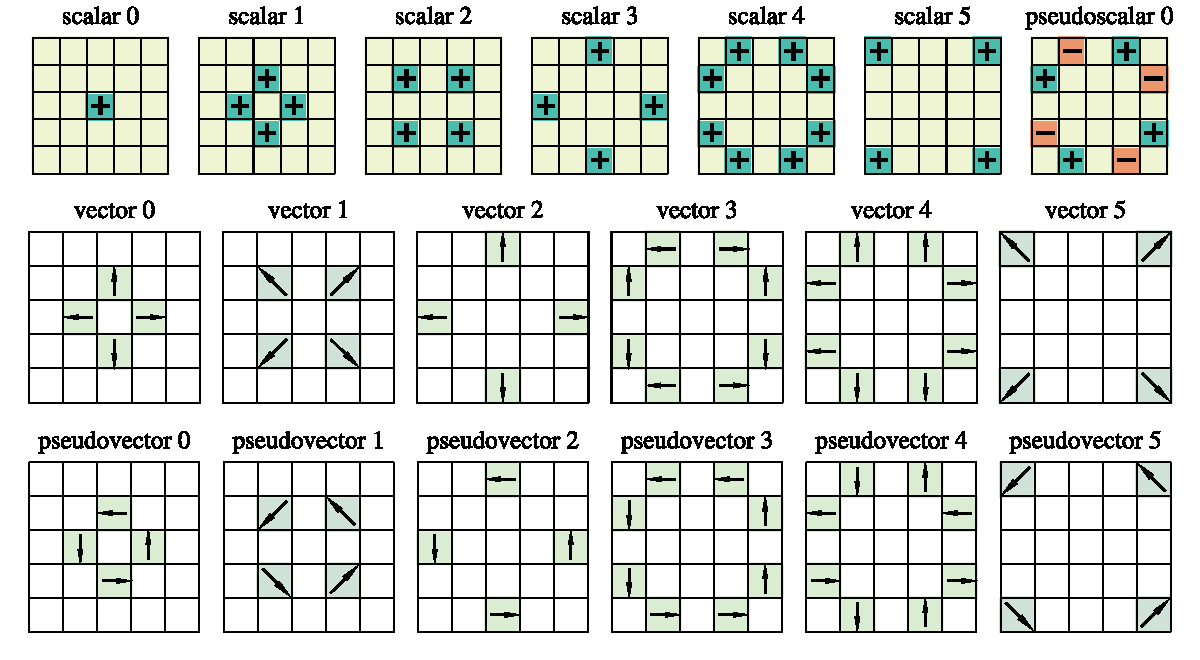
\includegraphics[width=\textwidth]{filters_m5.pdf}
    \end{minipage}
    \begin{minipage}{0.62\textwidth}
    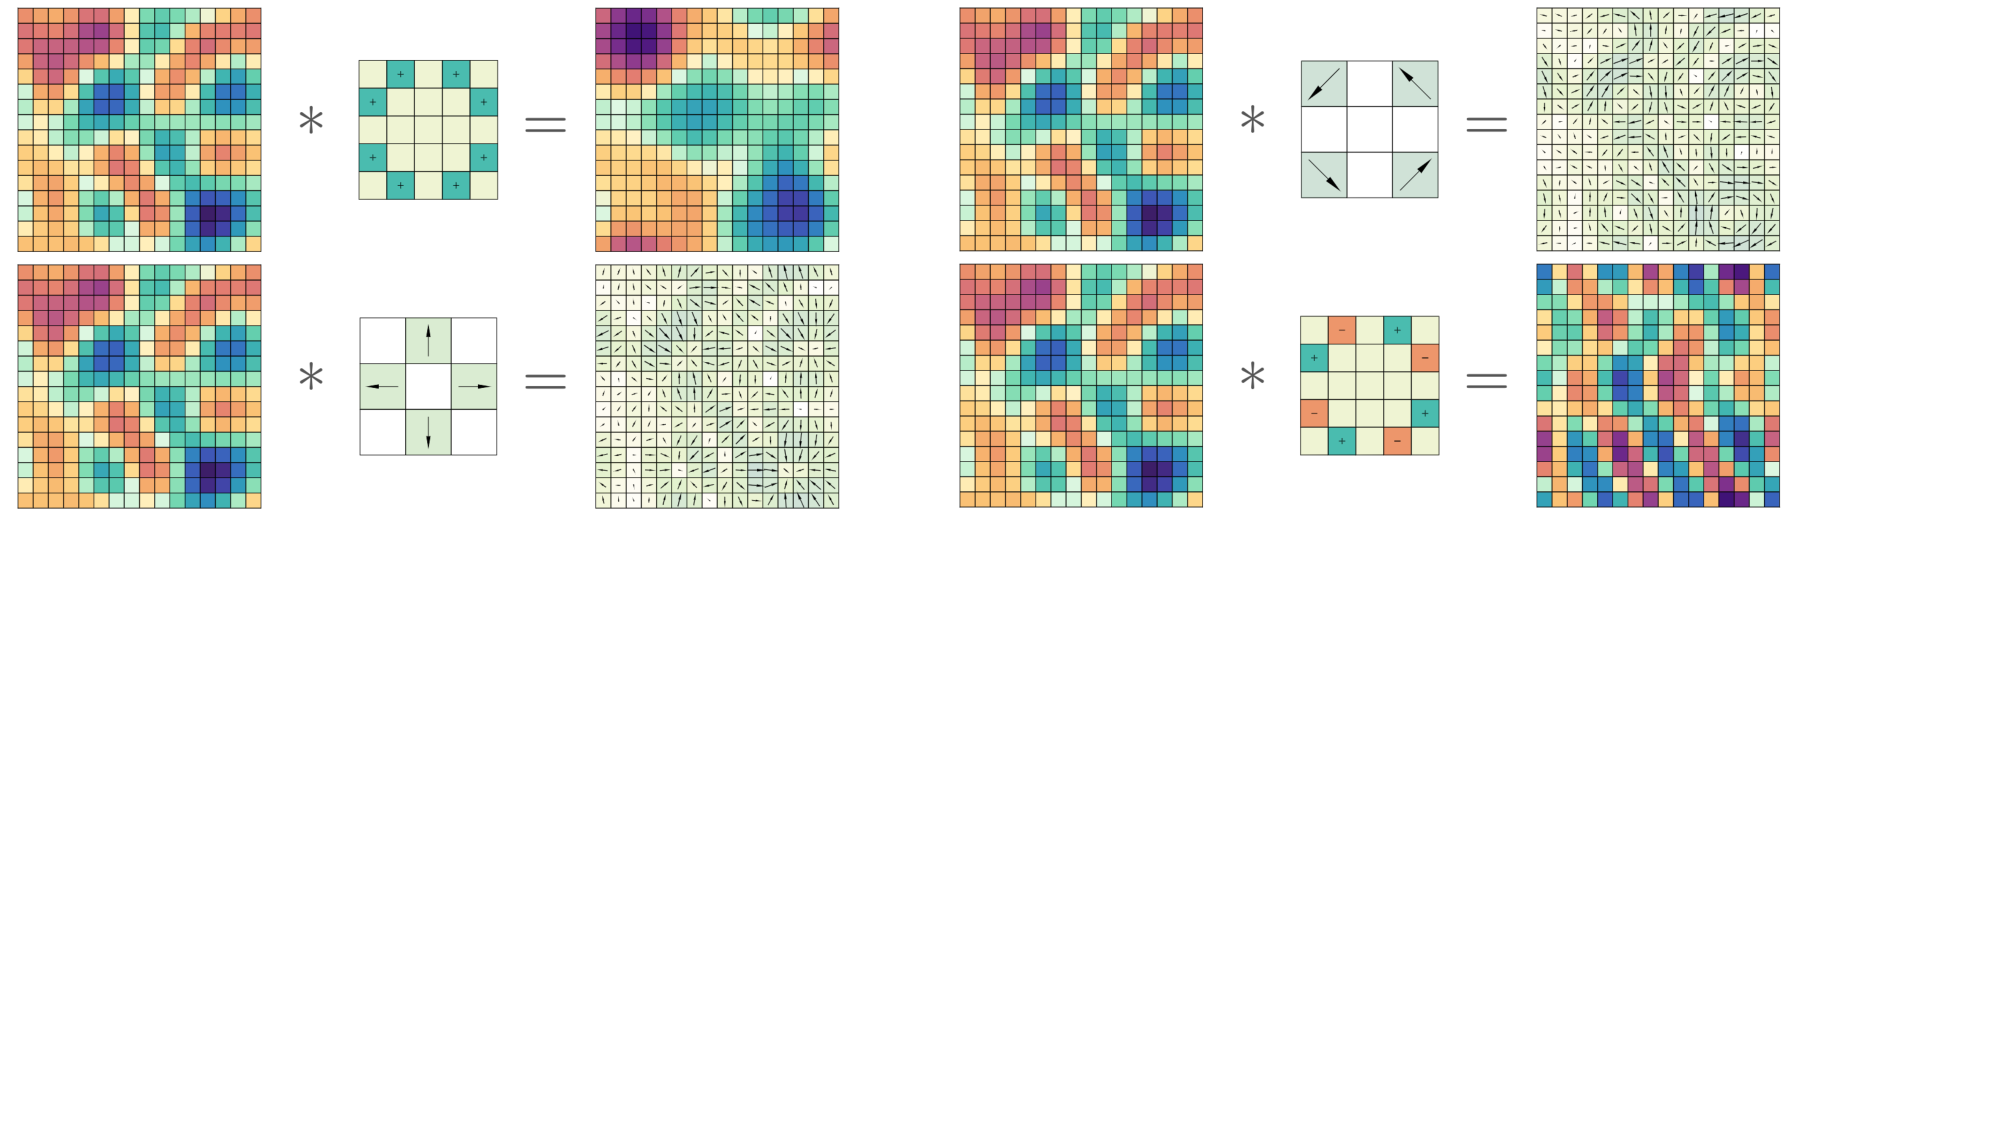
\includegraphics[width=\textwidth]{convs.pdf}
    \end{minipage}
    \vspace{-.3cm}
    \caption{(Left) The 5x5 scalar, pseudoscalar, vector, and pseudovector symmetric filters for 2-D images. (Right) Convolution of a scalar image with different geometric filters. Note the convolution with a scalar filter can be seen as the discretization of a diffusion operator, and the convolution with the vector filter resembles a discretization of the gradient. In general any symmetric discretization of any coordinate-free operator (gradient, divergence, curl) could be expressed in terms of our symmetric filters.}
    \label{fig.GINet}
\end{figure}

Any symmetric discretization of any coordinate-free operator (gradient, divergence, curl) could be expressed in terms of our symmetric filters. Therefore, this model is a natural tool to emulate the dynamics of physical models, arising from unknown (or partially known) PDEs, as done in the physics-informed machine learning literature \cite{karniadakis2021physics, hao2022physics}. It is an alternative approach to the more general theoretical frameworks from \cite{steerable, jenner2021steerable, bhardwaj2023steerable, clifford} that is specifically tailored to work for geometric images.   

SOLE: WE should discuss units covariance too.

We should discuss other representations of fields, but especially spherical harmonics.

\section{Red team}

In engineering disciplines, a ``red team'' is a team that, at an organization's behest, adversarially attacks the operations of the organization.
The organization learns from the successes of the red team, and gains confidence in its operations when it can defeat the red team.
This structure is designed specifically to build trust in the organization's practices.

In classical-physics contexts, the classical symmetries, including translation, rotation, boost, units covariance, particle permutations, and so on, lead to very precise predictions for simulation outputs given simple transformations of simulation inputs.
Thus these symmetries guide physics-informed adversarial attacks.
In addition, there are associated conservation laws in many cases, such as energy, angular momentum, linear momentum, mass, and so on.
All of these symmetries are in play in a passive sense in almost all natural-science and engineering problems: The underlying laws of physics obey all these symmetries exactly.
That said, most of them are broken an active sense: The boundary conditions, initial conditions, and problem contexts break the passive symmetries so they don't always appear actively in the input--output relationship of the simulations.

Each symmetry or conservation law in play leads to a vector for adversarial attack.
For example, a simulation on a square grid obeys a rotation symmetry where the inputs can be rotated through 90 degrees and the outputs should end up so rotated.
The adversarial attack against an emulator of that simulation is to find sets of initial conditions that maximize the difference between the output and the de-rotated output from a rotated input.
That is, the adversarial attack (created from a symmetry) is to search for emulator inputs that maximally violate the symmetry.

Symmetries and conservation laws are more valuable as they become more local, and as more of the simulation fields are tracked.
For example, momentum conservation is a symmetry that applies to every subvolume of every simulation, provided that the simulation outputs are rich enough to track stress fields.
This is because the momentum conservation can be seen as a balance between the rate of change of the local momentum density and the divergence of the local stress tensor field.
Thus some symmetries lead to very high dimensional predictions or predictions that apply to essentially every grid cell in a simulation at every time step.
When an emulator produces sufficient output, there might be very detailed attack strategies against that emulator.
Again, the attack would be to search for inputs such that there is a maximal violation of the local prediction from the conservation law.

HOGG: How would attack help us?

HOGG: When are you safer and less safe wrt attack?

HOGG: Concept of enforcing Lipschitz on the inputs??

\section{Emulation of cosmological fields}

Recent works in computational cosmology employ deep neural networks to enhance low-resolution dark matter-only simulations, generating super-resolution realizations that agree remarkably well with the full simulation counterparts on their statistical properties and are orders of magnitude faster \cite{li2021ai, ni2021ai}. 

In general, the n-body simulations are initialized on a cubic lattice, with the initial conditions encoded as small position and velocity displacements away from the perfect cubic lattice. Thus the points in the n-body simulation start on a regular grid, and can be identified throughout the simulation evolution with their initial grid locations.

For instance, in \cite{li2021ai} the evolution of the n-body simulation is represented with a 3D grid with 3 channels (each
channel corresponds to one component of the displacement vector). A deep learning model, based on StyleGAN2 \cite{karras2020analyzing}, takes the low resolution particle displacements as input, and outputs a possible realization of their high resolution counterparts. They use data augmentation to regularize the model to be approximately $SO(3)$-equivariant. 

We propose to improve cosmological models such as \cite{li2021ai, ni2021ai} by using a 3D geometric image to represent positions (and velocities) instead of a 3D grid with 3 (or 6) independent channels. The evolution equations are independent of orientation and position (they are coordinate free!), so they are implementable as an GeometricImageNet model. Current state-of-the-art on such emulators do not enforce any symmetries beyond simple translation symmetry or data augmentation; they do not enforce O(3) symmetry or Lorentz invariance or Hamiltonian phase-space-density conservation.

\section{Emulation of ocean dynamics}

Climate and climate change are studied through coupled models of the ocean and atmosphere. For ocean dynamics, the primitive equations are derived from the Navier-Stokes equations on a sphere, considering the impact of Earth's rotation and complex boundary conditions. Additional assumptions include hydrostatic balance between the ocean and atmosphere, incompressibility of the fluid, and small temperature and density variations. Under these assumptions, the resulting equations are known as a Boussinesq approximation, where the fluid density remains nearly constant, except for buoyancy effects, which are accounted for by a buoyancy term. The resulting differential equations are of course independent of the coordinate system.

The Geophysical Fluid Dynamics Laboratory (GFDL) of the National Oceanic and Atmospheric Administration produce datasets where models are corrected with real observations \cite{obrien2004gfdl, rutledge2006nomads, delworth2020spear}. 
For instance the CM2.6 has a resolution of 10 km for the ocean with 50 vertical levels and a sea ice model, and 50 km for the atmosphere. 

Although it is essential for addressing certain climate problems \cite{jong2023increases, pascale2020increasing, zhou2019toward}, the increased realism of high resolution modeling comes at a high computational cost. Consequently, high resolution climate models are used in conjunction with other tools, including machine learning, that are more amenable to exploring long time scales or focus on incorporating comprehensive climate processes. 

We propose GeometricImageNet as a tool with the right inductive bias to incorporate in the existing computational pipelines, as a replacement for CNNs. WHAT ARE THE SCIENTIFIC GOALS OF THE OCEAN SIMULATIONS?



% \renewcommand\refname{References Cited} % if you want to change the name
\bibliographystyle{IEEEtran}
\bibliography{emulator}

\appendix
\section{Technical details of what now?}

\section{Simulation-based inference}
HOGG: Explain simulation-based inference here, and why it needs so many damned simulations.

\section{Delete me, but only after use}
This white paper is addressing the ONR program ``Applied and Computational Analysis''.%
\footnote{\url{https://www.nre.navy.mil/organization/departments/code-31/division-311/applied-and-computational-analysis}}

Here's a list of possible topics.
Let's brainstorm for now (that is, be ``yes, and'' rather than ``no, but''), and be more editorial later.
\begin{itemize}
    \item Ordinary differential equations with geometric objects.
    \item Partial differential equations with geometric fields (eg, Drummond's)
    \item specific applications to Cosmology (eg, Connor; a nonlinear dynamics problem) or Oceans (eg, Zanna; a multi-phase fluids problem with and mixing and transport)
    \item Spectral-method or basis-function generalizations of Wilson's stuff.
    \item Generalization of Wilson's model to lightly curved surfaces, by instantiating the local metric (or a metric offset) at every pixel.
    \item Explicit generalization of a CNN to diffeomorphisms (possibly restricted in some ways).
    \item Contrastive learning with approximate or exact symmetries in either the data space or the latent space or both.
    \item Demonstrate that enforcing passive symmetries can help, even when the problem is not actively symmetric, or not! Or maybe in pre-processing or scaling or normaliztions. See the section in the passive symmetries paper about normalization.
    \item Possibly draw connections to acoustics in nonlinear environments, maybe? Or find an acoustics problem?
    \item Enforce conservation laws locally at the pixel level, or spectral component level, in the oceans problem.
    \item 
\end{itemize}

\end{document}
